%compiling with XeLaTeX
\documentclass[digital, %colors on
			   %print,  %for printing
			   %twoside, %turn off for digital version
			   openright, %chapter always start on the right page
			   parskip=half,
			   11pt]{mythesis}

\usepackage{bbold}


\begin{document}
\pagestyle{plain}

\section*{Quark-Self Energy Diagram using Spectral Representations}
 The relevant diagram for our computation of the quark spectral function is the one-loop contribution to the Dyson-Schwinger equation for the (inverse) quark propagator:
 \begin{align}
\bigg(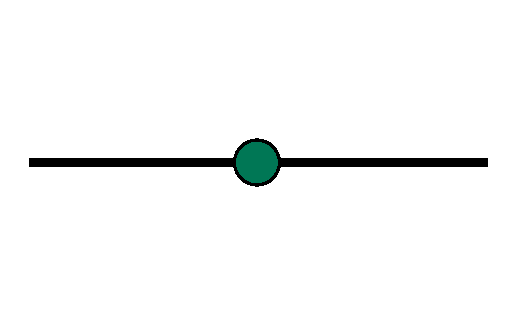
\includegraphics[scale=0.4, valign=c]{diagram/full_quark_propagator}\bigg)^{-1} = 
\bigg(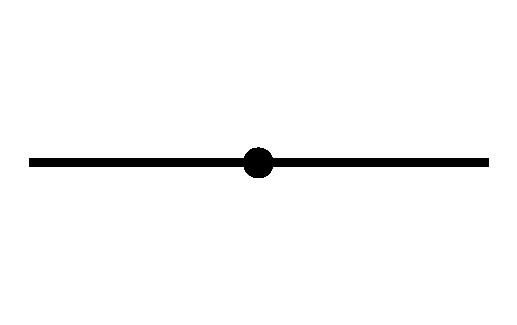
\includegraphics[scale=0.4, valign=c]{diagram/bare_quark_propagator.pdf}\bigg)^{-1} - 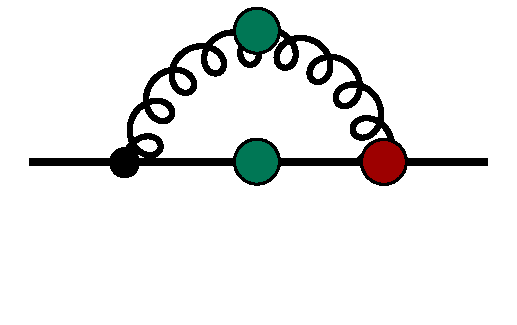
\includegraphics[scale=0.4, valign=c]{diagram/quark_self_energy}
\end{align}
 
Applying the Feynman rules for Landau gauge QCD ($\xi = 0$) from the lecture notes we find\footnote{Note that we work in a classical vertex approximation, i.\,e. $\Gamma^{(3)}_{q\bar{q}A} \equiv S^{(3)}_{q\bar{q}A}$.}:
\begin{align*}
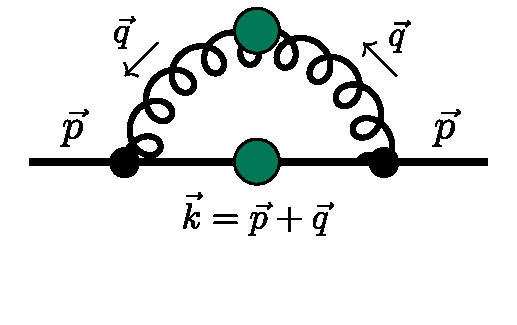
\includegraphics[scale=0.5, valign=c]{diagram/quark_self_energy_classical} := \Sigma(p) &= (-ig)^2 T^{a}T^b \int \frac{\dd^4 q}{(2\pi)^4}\ \delta_{ab}\ \Pi^{\mu\nu}_{\bot}(q) G_A(q)\gamma_{\mu}G_F(p+q)\gamma_{\nu}
\end{align*}
with the transverse projection operator defined via
\begin{equation}
	\Pi^{\mu\nu}_{\bot}(p) = \delta^{\mu\nu} - \frac{p^{\mu}p^{\nu}}{p^2},
\end{equation}
and the respective spectral representations of the gluon propagator $G_A$ and the fermionic quark propagator $G_F$, given by

\begin{equation}
\begin{aligned}
G_F(p) &=\slashed{p} G_{1}(p)+G_{2}(p)  \\
&= \slashed{p} \int_{0}^{\infty} \frac{\dd \lambda}{\pi} \frac{\lambda\rho_{1}(\lambda)}{p^{2}+\lambda^2}+\int_{0}^{\infty} \frac{\dd \lambda}{\pi} \frac{\lambda\rho_{2}(\lambda)}{p^{2}+\lambda^2},
\end{aligned}
\end{equation}
and
\begin{align} 
G_A(p)&=\int_{0}^{\infty} \frac{\dd \lambda_A}{\pi} \frac{\lambda_A\rho_A(\lambda_A)}{p^{2}+\lambda_A^{2}}.
\end{align}
In total we are left with the following expression for the amputated diagram:\\
\color{MScRed}  We first need to take care of additional factors arising from permuting the second gamma matrix with the one contained in the fermion propagator. We use
\begin{equation}
	\left\{ \gamma^{\mu},\gamma^{\nu}\right\} = 2\delta^{\mu\nu}.
\end{equation} \newpage
\normalcolor
After carefully permuting all relevant terms we are left with 
\begin{equation}
	\begin{aligned}
		\Sigma_{\mathrm{vec}}(p) &\sim \int_q \left(\color{MScRed}(3-d)\slashed{p}\normalcolor + \left(\color{MScBlue}(1-d)\normalcolor - \color{MScGreen}2\ \frac{p\cdot q}{q^2}\normalcolor\right)\slashed{q}\right)\int_{\lambda_A,\lambda} \frac{\lambda_A\rho(\lambda_A)}{q^2 + \lambda_A^2} \frac{\lambda\rho_1(\lambda)}{(p+q)^2 + \lambda^2} \\[0.5em]
		\Sigma_{\mathrm{scal}}(p) &\sim \int_q (d-1)\int_{\lambda_A,\lambda} \frac{\lambda_A\rho(\lambda_A)}{q^2 + \lambda_A^2} \frac{\lambda\rho_2(\lambda)}{(p+q)^2 + \lambda^2}
	\end{aligned}
\end{equation}
where we have split the total diagram into its Dirac vector and scalar part, i.\,e.
\begin{equation}
	\Sigma(p) = (-ig)^2 C_f \left(\Sigma_{\mathrm{vec}}(p) + \Sigma_{\mathrm{scal}}(p)  \right).
\end{equation}
The only nontrivial contribution (that was missing before!!!) is the one that is highlighted in green since it provides additional momentum structure that was missing before! But let's first discuss the other two terms. Ignoring the spectral integrals first we quickly find
\begin{equation}
	(3-d)\slashed{p} \int_q \frac{1}{q^2 + \lambda_A^2}\frac{1}{(p+q)^2 + \lambda^2} = (3-d)\slashed{p}\int_{x,q} \frac{1}{\left[q^2 + \Delta_1\right]^2}
\end{equation}
with 
\begin{equation}
	\Delta_1 = x(1-x)p^2 + (1-x)\lambda_A^2 + x\lambda^2,
\end{equation}
after Feynman parameter decomposition and shifting the loop momentum $q \rightarrow q-xp$.\\
For $\Sigma_{\mathrm{scal}}$ we get the same result (with the correct prefactor $(d-1)$ of course.) The term highlighted in blue is a bit trickier since it involves another factor of $q^{\alpha}$: 
\begin{equation}
\begin{aligned}
	(1-d)\gamma_{\alpha} \int_q q^{\alpha} \frac{1}{q^2 + \lambda_A^2}\frac{1}{(p+q)^2 + \lambda^2} &= (1-d)\gamma_{\alpha}\int_{x,q} (q^{\alpha} - xp^{\alpha})\frac{1}{\left[q^2 + \Delta_1\right]^2}\\
	&= (d-1)\slashed{p}\int_{x,q}\frac{x}{\left[q^2 + \Delta_1\right]^2}.
	\end{aligned}
\end{equation}
Here we used that all integrations involving an odd power of $q$ are zero. Following the same line of arguments we can also simplify the third relevant term:
\begin{equation}
	\begin{aligned}
		-2\gamma_{\alpha} \int_q q^{\alpha}\frac{p\cdot q}{q^2} \frac{1}{q^2 + \lambda_A^2}\frac{1}{(p+q)^2 + \lambda^2} = -2\frac{\gamma_{\alpha}p_{\beta}}{\lambda_A^2}\int_q\left\{\left(\frac{ q^{\alpha}q^{\beta}}{q^2 ((p+q)^2 + \lambda^2)}\right)\right.\\ \left. - \left(\frac{ q^{\alpha}q^{\beta}}{(q^2 + \lambda_A^2)((p+q)^2 + \lambda^2)}\right)\right\}
	\end{aligned}
\end{equation}
Now we can again perform the Feynman trick and shift the loop momentum to obtain:
\begin{equation}
	\cdots = -2\frac{\gamma_{\alpha}}{\lambda_A^2}\int_{x,q}\left\{ \left((p\cdot q)q^{\alpha} + x^2p^2p^{\alpha}\right)\left(\frac{1}{\left[q^2 + \Delta_2\right]^2} - \frac{1}{\left[q^2 + \Delta_1\right]^2}\right) \right\}
\end{equation}
where we again discarded all terms that were odd in $q$. Additionally we defined
\begin{equation}
	\Delta_2 = \Delta_1 - (1-x)\lambda_A.
\end{equation}
For the first part we symmetrize the momenta according to 
\begin{equation}
	q^{\alpha}q^{\beta} = \frac{1}{d}\delta^{\alpha\beta}q^2,
\end{equation}
which is valid under the integral, and therefore find in total:
\begin{equation}
	\cdots = -2\frac{\slashed{p}}{\lambda_A^2}\int_{x,q}\left\{\frac{1}{d}\left(\frac{q^2}{\left[q^2 + \Delta_2\right]^2} - \frac{q^2}{\left[q^2 + \Delta_1\right]^2}\right) + p^2x^2\left(\frac{1}{\left[q^2 + \Delta_2\right]^2} - \frac{1}{\left[q^2 + \Delta_1\right]^2}\right)\right\}
\end{equation}
Now we store all prefactors in front of all terms of different powers in $q$ in our notebook and perform the \enquote{trivial} momentum integrations. 
\section*{Momentum Integration}

The momentum integration can now we performed using standard integration formulae known in the context of dimensional regularization, the regularization scheme of our choice. Therefore, the  dimensionality of the integral is promoted to $d= 4 -2\varepsilon$. To account for this we need to introduce a factor of $\mu^{2\varepsilon}$ under the integral.

In general (cf. Peskin/Schroeder) it holds true, that 
\begin{equation}
\begin{aligned}
	\int \frac{\dd^d q}{(2\pi)^d} \frac{1}{\left[q^2 + \Delta\right]^2} &\overset{\phantom{(*)}}{=}  \frac{1}{(4\pi)^{\frac{d}{2}}} \frac{\Gamma(2-\frac{d}{2})}{\Gamma(2)} \Delta^{\frac{d}{2}-2} \\
	&\overset{(*)}{=} \frac{1}{(4\pi)^{2}}\left(\frac{1}{\varepsilon} - \operatorname{log}\Delta - \gamma_{\mathrm{E}} + \operatorname{log} 4\pi + \operatorname{log} \mu^2 + \mathcal{O}(\varepsilon)\right)\\
	&\overset{\phantom{(*)}}{=} \frac{1}{(4\pi)^{2}}\left(\frac{1}{\varepsilon} - \operatorname{log}\Delta + \operatorname{log}\left(\frac{4\pi\mu^2}{\operatorname{e}^{\gamma_{\mathrm{E}}}}\right)   + \mathcal{O}(\varepsilon)\right),
	\end{aligned}
\end{equation}
where we went to $d= 4 -2\varepsilon$ and expanded the relevant quantities up to lowest order in $\varepsilon$ in the limit $\varepsilon\rightarrow 0$. This isolates the divergence of the diagram in the $\frac{1}{\varepsilon}$-term which is discarded, as usual. Note that we still need to renormalize the spectral integrals later on, since we swapped the integration order which is only allowed for finite integrands!\\
The second important integral is solved analogously:
\begin{equation}
\begin{aligned}
	\int \frac{\dd^d q}{(2\pi)^d} \frac{q^2}{\left[q^2 + \Delta\right]^2} &=  \frac{1}{(4\pi)^{\frac{d}{2}}} \frac{\Gamma(1+\frac{d}{2})\Gamma(1-\frac{d}{2})}{\Gamma(\frac{d}{2})\Gamma(2)} \Delta^{\frac{d}{2}-1} \\
	&= \frac{1}{(4\pi)^{\frac{d}{2}}}\left(\frac{d}{2-d}\right)\Gamma\big(2-\frac{d}{2}\big) \Delta\cdot\Delta^{\frac{d}{2}-2} \\
	&= \frac{-2}{(4\pi)^{2}}\Delta\left(\frac{1}{\varepsilon} +\frac{1}{2}- \operatorname{log}\Delta - \gamma_{\mathrm{E}} + \operatorname{log} 4\pi + \operatorname{log} \mu^2 + \mathcal{O}(\varepsilon)\right)\\
	&= \frac{-2}{(4\pi)^{2}}\Delta\left(\frac{1}{\varepsilon} +\frac{1}{2} - \operatorname{log}\Delta + \operatorname{log}\left(\frac{4\pi\mu^2}{\operatorname{e}^{\gamma_{\mathrm{E}}}}\right)   + \mathcal{O}(\varepsilon)\right),
	\end{aligned}
\end{equation}
where we used that $\Gamma(x+1)=x\Gamma(x)\ \forall x\in \mathbb{C}$.
This allows us to recast the entire integrands in the following form:
\begin{equation}
\begin{array}{c}
I_{\mathrm{vec}}\left(p, \lambda_{A}, \lambda\right)=\left(\frac{1}{\varepsilon}+\log \left(\frac{4 \pi \mu^{2}}{e^{\gamma_{\mathrm{E}}}}\right)\right) \sum\limits_{i=0}^{2} \frac{\alpha_{i}-\beta_{i}}{i+1} 
-\mathlarger{\int}\limits_{x} \sum\limits_{i=0}^{2} x^{i}\left(\alpha_{i} \log \Delta_{1}-\beta_{i} \log \Delta_{2}\right)+\mathcal{O}(\varepsilon).
\end{array}
\end{equation}
\begin{equation}
\begin{array}{c}
I_{\mathrm{scal}}\left(p, \lambda_{A}, \lambda\right)=\left(\frac{1}{\varepsilon}+\log \frac{4 \pi \mu^{2}}{e^{\gamma_{\mathrm{E}}}}\right) \gamma_0
-\mathlarger{\int}\limits_{x} \gamma_{0} \log \Delta_{1} +\mathcal{O}(\varepsilon).
\end{array}
\end{equation}
The respective coefficients are now the reordered coefficients in front of the terms in different powers of the Feynman parameter $x$. They are not displayed here due to their length, but they are stored in the corresponding Mathematica notebook.


\section*{Feynman Parameter Integration}
In the next step, the respective Feynman integrals can be performed. We use standard Mathematica integration routines and compare the result with numerical integration to avoid making mistakes. We do not present the lengthy expressions here, they can be found in the corresponding notebook \texttt{newterms.nb}. The relevant integrals are  
\begin{align}
	f_i(p,\lambda_A, \lambda) &\sim \int_0^1 \dd x\ x^{i} \operatorname{log}\Delta_1 \\
g_i(p,\lambda_A, \lambda) &\sim \int_0^1 \dd x\ x^{i} \operatorname{log}\Delta_2
\end{align}
with $i$ ranging from 0 to 2.
\section*{Comparison with perturbative results }
To benchmark our results we need to compare them to known perturbative expressions of the diagram. How can we compare this? $\rightarrow$ Get rid of the spectral integrals by imposing the \enquote{classical} spectral functions that reproduce the classical, perturbative propagators:
\begin{equation}
	G_F(p) = \frac{i\slashed{p}-m_q}{p^2+m_q^2}
\end{equation}
and 
\begin{equation}
	G_A(p) = \frac{1}{p^2}
\end{equation}
\color{MScRed} We have to pay attention to the fact, that we are working with a spectral function of a linear argument $\lambda$. We therefore have to be careful with the correct implementation of the Dirac delta function. We want to make use of the definition of the delta function of a composed function:
\begin{equation}
	(\delta\circ f)(x) = \sum_i^{N_{\mathrm{roots}}}\frac{\delta(x-x_i)}{\abs{f'(x_i)}}.
\end{equation}
This gives the following result for our specific problem:
\begin{equation}
	\delta(x^2-a^2) = \frac{1}{\abs{2a}}\delta(x-a).
\end{equation}
\normalcolor
Applying the considerations made above, we find:
\begin{equation}
	\begin{aligned}
		\rho_{1,\mathrm{class}}(\lambda) &= 2\pi i\ \eval{\frac{\delta(\lambda-m_q)}{2\lambda}}_{\lambda=m_q}\\
		\rho_{2,\mathrm{class}}(\lambda) &= 2\pi m_q\ \eval{\frac{\delta(\lambda-m_q)}{2\lambda}}_{\lambda=m_q}.
	\end{aligned}
\end{equation}
The same ideas lead us to the following result for the massless gluon spectral function
\begin{equation}
	\rho_{A,\mathrm{class}}(\lambda_A) = 2\pi\ \eval{\frac{\delta(\lambda_A)}{2\lambda_A}}_{\lambda_A=0}.
\end{equation}
\color{MScRed} I asked myself, if the cancellation of the respective $\lambda$'s in the denominators with the the ones appearing in front of the spectral functions in the nominator is \enquote{trivial} or if we have to be careful with some non-trivial cancellations due to the specific evaluation at the pole masses.\\
\textbf{Resolved:} I thought in more detail about the properties of the $\delta$-function and came to the conclusion, that using 
\begin{equation}
	1
\end{equation} 
\normalcolor
\section*{Analytic Continuation of the Integrands}
To be able to access the spectral functions we need to perform an analytical continuation $p_{0} \rightarrow-i(\omega+i \epsilon)$. Be aware that Mathematica does NOT take the correct limit $\varepsilon\rightarrow 0^+$, but it turns out that the right way of continuing the $\operatorname{log}$-terms is given by:
\begin{equation}
	\lim _{\varepsilon \rightarrow 0^+} \log (x+i \varepsilon)=\log x+i \pi \theta(-x)
\end{equation}
\color{MScRed} ToDo: Plots for showing the correct continuation. \normalcolor
\section*{A few Comments on the Gluon Spectral Function}
\begin{figure}[H]
	\centering
	\includegraphics[scale = 0.25]{plots/gluon_specfunc}
	\caption{Gluon spectral function (decoupling) from Nicolas/Jan used for our computation.}
\end{figure}
\section*{Some thoughts on the structure of the quark propagator DSE}
We know that 
\begin{equation}
G_F(p) = \slashed{p} \int_{0}^{\infty} \frac{\dd \lambda}{\pi} \frac{\lambda\rho_{1}(\lambda)}{p^{2}+\lambda^2}+\int_{0}^{\infty} \frac{\dd \lambda}{\pi} \frac{\lambda\rho_{2}(\lambda)}{p^{2}+\lambda^2},
\end{equation}
which implies, that the  inverse quark propagator should be of the form:
\begin{equation}
	G_F^{-1}(p) = A(p)\cdot\slashed{p} + B(p)\cdot\mathbb{1},
\end{equation}
where the unit matrix has to be understood as the identity in Dirac space. This allows us to conclude, that
\begin{align}
\rho_1 &= \rho_1(A(p), B(p)) 	\\
\rho_2 &= \rho_2(A(p), B(p)) 
\end{align}
In can be projected on its Dirac vector and scalar parts by multiplying it with either $\slashed{p}$ or $\mathbb{1}$ and performing the corresponding traces: 

\begin{align}
\rho_1 &= \operatorname{Tr} \left[ \slashed{p}\cdot 2\Im G_F^{-1}(-i(\omega + i\varepsilon))\right]	\\
\rho_2 &= \operatorname{Tr} \left[ \mathbb{1}\cdot 2\Im G_F^{-1}(-i(\omega + i\varepsilon))\right]
\end{align}


\end{document}